\let\mypdfximage\pdfximage
\def\pdfximage{\immediate\mypdfximage}
\documentclass[10pt,onecolumn,letterpaper]{article}
%\usepackage[latin1]{inputenc}
\usepackage{epstopdf}
\usepackage{iccv}
\usepackage{times}
\usepackage{epsfig}
\usepackage{graphicx}
\usepackage{grffile}
\usepackage{amsmath}
\usepackage{amssymb}
\usepackage{amsmath}
\usepackage{amsfonts}
\usepackage{subfigure}
\usepackage{nonfloat}
\usepackage{url}
%\usepackage[colorlinks=true, linkcolor=green, pagebackref]{hyperref}
\usepackage{textcomp} % for textonehalf
\usepackage{longtable}
\usepackage{wrapfig}
\graphicspath{{imgs/voxpop/}{imgs/bb_input/}{imgs/bb_renders/}{imgs/turn_table_iccv_pdf_01/}{imgs/turn_table_views/}{imgs/}{imgs/training_images/}{imgs/new_bb/}}

\usepackage{xspace}
\renewcommand*{\eg}{e.g.\@\xspace}
\renewcommand*{\ie}{i.e.\@\xspace}
\newcommand*{\ea}{et al.\@\xspace}
\renewcommand*{\vs}{vs.\@\xspace}

%\cvprfinalcopy % *** Uncomment this line for the final submission

\def\iccvPaperID{351} % *** Enter the CVPR Paper ID here
\def\httilde{\mbox{\tt\raisebox{-.5ex}{\symbol{126}}}}

% \renewcommand{\paragraph}{\vspace{2pt}\noindent\textbf}

% \let\stdsection\section
% \renewcommand\section{\newpage\stdsection}

\title{Structured Prediction of Unobserved Voxels From a Single Depth Image: Supplementary Material}

\begin{document}

\maketitle

\tableofcontents



%%%%%%%%%%%%%%%%%%%%%%%%%%%%%%%%%%%%%%%%%%%%%%%%%%%%%%%%
\newpage
\section{`BigBIRD' turntable dataset: Additional results}

Figure 1 shows additional results from the BigBIRD turntable dataset.
We note that we are able to gain good reconstructions even where the object suffers from heavy self-occlusions  (e.g. (a) and (d)).
However, where much of the data is missing through the height of the object, we can fail to recover the main bulk (e.g. (c) and (e)).
We note that the baseline algorithms can also perform poorly under such conditions.
% , under- or over- predicting the volume.

\newcommand{\turnheight}{0.12\columnwidth}
\begin{figure*}[h!]
\begin{tabular}{cccccc}
    (a) \includegraphics[height=\turnheight, clip=true, trim=20 30 30 5]{ritz_crackers_NP3_0.png} &
\includegraphics[height=\turnheight, clip=true, trim=50 30 10 5]{a.png} &
\includegraphics[height=\turnheight, clip=true, trim=60 30 30 5]{ritz_crackers_NP3_0.mat_gt_view_180.png} &
\includegraphics[height=\turnheight, clip=true, trim=60 30 30 5]{ritz_crackers_NP3_0.mat_bb_view_180.png} &
\includegraphics[height=\turnheight, clip=true, trim=60 30 30 5]{ritz_crackers_NP3_0.mat_zheng_view_180.png} &
\includegraphics[height=\turnheight, clip=true, trim=60 30 30 5]{ritz_crackers_NP3_0.mat_oma_view_180} \\
(b) \includegraphics[height=\turnheight, clip=true, trim=20 30 30 5]{vo5_extra_body_volumizing_shampoo_NP2_216.png} &
\includegraphics[height=\turnheight, clip=true, trim=60 30 10 5]{b.png} &
\includegraphics[height=\turnheight, clip=true, trim=60 30 30 5]{vo5_extra_body_volumizing_shampoo_NP2_216.mat_gt_view_0.png} &
\includegraphics[height=\turnheight, clip=true, trim=60 30 30 5]{vo5_extra_body_volumizing_shampoo_NP2_216.mat_bb_view_0.png} &
\includegraphics[height=\turnheight, clip=true, trim=60 30 30 5]{vo5_extra_body_volumizing_shampoo_NP2_216.mat_zheng_view_0.png} &
\includegraphics[height=\turnheight, clip=true, trim=60 30 30 5]{vo5_extra_body_volumizing_shampoo_NP2_216.mat_oma_view_0} \\
(c) \includegraphics[height=\turnheight]{NP4_0.jpeg} &
\includegraphics[height=\turnheight, clip=true, trim=60 30 10 5]{c.png} &
\includegraphics[height=\turnheight, clip=true, trim=60 30 30 5]{sunkist_fruit_snacks_mixed_fruit_NP4_0.mat_gt_view_180.png} &
\includegraphics[height=\turnheight, clip=true, trim=60 30 30 5]{sunkist_fruit_snacks_mixed_fruit_NP4_0.mat_bb_view_180.png} &
\includegraphics[height=\turnheight, clip=true, trim=60 30 30 5]{sunkist_fruit_snacks_mixed_fruit_NP4_0.mat_zheng_view_180.png} &
\includegraphics[height=\turnheight, clip=true, trim=60 30 30 5]{sunkist_fruit_snacks_mixed_fruit_NP4_0.mat_oma_view_180} \\
(d) 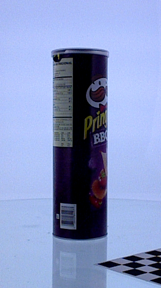
\includegraphics[height=\turnheight, clip=true, trim=20 30 30 5]{pringles_bbq_NP1_312.png} &
\includegraphics[height=\turnheight, clip=true, trim=60 30 10 5]{d.png} &
\includegraphics[height=\turnheight, clip=true, trim=60 30 30 5]{pringles_bbq_NP1_312.mat_gt_view_180.png} &
\includegraphics[height=\turnheight, clip=true, trim=60 30 30 5]{pringles_bbq_NP1_312.mat_bb_view_180.png} &
\includegraphics[height=\turnheight, clip=true, trim=60 30 30 5]{pringles_bbq_NP1_312.mat_zheng_view_180.png} &
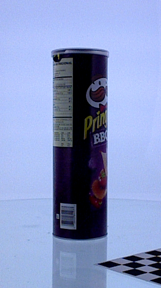
\includegraphics[height=\turnheight, clip=true, trim=60 30 30 5]{pringles_bbq_NP1_312.mat_oma_view_180} \\
% (g) \includegraphics[height=\turnheight, clip=true, trim=20 30 30 5]{pringles_bbq_NP4_0.png} &
% \includegraphics[height=\turnheight, clip=true, trim=60 30 30 5]{pringles_bbq_NP4_0_visible_pixels_view_0.png} &
% \includegraphics[height=\turnheight, clip=true, trim=60 30 30 5]{pringles_bbq_NP4_0_gt_view_0.png} &
% \includegraphics[height=\turnheight, clip=true, trim=60 30 30 5]{pringles_bbq_NP4_0_bb_view_0.png} &
% \includegraphics[height=\turnheight, clip=true, trim=60 30 30 5]{pringles_bbq_NP4_0_zheng_view_0.png} &
% \includegraphics[height=\turnheight, clip=true, trim=60 30 30 5]{pringles_bbq_NP4_0_oma_view_0} \\
(e) \includegraphics[height=\turnheight, clip=true, trim=20 30 30 5]{spongebob_squarepants_fruit_snaks_NP3_312.png} &
\includegraphics[height=\turnheight, clip=true, trim=20 30 20 5]{e.png} &
\includegraphics[height=\turnheight, clip=true, trim=60 30 30 5]{spongebob_squarepants_fruit_snaks_NP3_312.mat_gt_view_270.png} &
\includegraphics[height=\turnheight, clip=true, trim=60 30 30 5]{spongebob_squarepants_fruit_snaks_NP3_312.mat_bb_view_270.png} &
\includegraphics[height=\turnheight, clip=true, trim=60 30 30 5]{spongebob_squarepants_fruit_snaks_NP3_312.mat_zheng_view_270.png} &
\includegraphics[height=\turnheight, clip=true, trim=60 30 30 5]{spongebob_squarepants_fruit_snaks_NP3_312.mat_oma_view_270} \\
(f) \includegraphics[height=\turnheight, clip=true, trim=20 30 30 5]{sunkist_fruit_snacks_mixed_fruit_NP3_0.png} &
\includegraphics[height=\turnheight, clip=true, trim=60 30 10 5]{f.png} &
\includegraphics[height=\turnheight, clip=true, trim=60 30 30 5]{sunkist_fruit_snacks_mixed_fruit_NP3_0.mat_gt_view_180.png} &
\includegraphics[height=\turnheight, clip=true, trim=60 30 30 5]{sunkist_fruit_snacks_mixed_fruit_NP3_0.mat_bb_view_180.png} &
\includegraphics[height=\turnheight, clip=true, trim=60 30 30 5]{sunkist_fruit_snacks_mixed_fruit_NP3_0.mat_zheng_view_180.png} &
\includegraphics[height=\turnheight, clip=true, trim=60 30 30 5]{sunkist_fruit_snacks_mixed_fruit_NP3_0.mat_oma_view_180} \\
(g) \includegraphics[height=\turnheight, clip=true, trim=20 30 30 5]{red_bull_NP3_0.png} &
\includegraphics[height=\turnheight, clip=true, trim=60 30 10 5]{g.png} &
\includegraphics[height=\turnheight, clip=true, trim=60 30 30 5]{red_bull_NP3_0.mat_gt_view_180.png} &
\includegraphics[height=\turnheight, clip=true, trim=60 30 30 5]{red_bull_NP3_0.mat_bb_view_180.png} &
\includegraphics[height=\turnheight, clip=true, trim=60 30 30 5]{red_bull_NP3_0.mat_zheng_view_180.png} &
\includegraphics[height=\turnheight, clip=true, trim=60 30 30 5]{red_bull_NP3_0.mat_oma_view_180} \\
(h) \includegraphics[height=\turnheight, clip=true, trim=20 30 30 5]{tapatio_hot_sauce_NP3_216.png} &
\includegraphics[height=\turnheight, clip=true, trim=60 30 10 5]{h.png} &
\includegraphics[height=\turnheight, clip=true, trim=60 30 30 5]{tapatio_hot_sauce_NP3_216.mat_gt_view_0.png} &
\includegraphics[height=\turnheight, clip=true, trim=60 30 30 5]{tapatio_hot_sauce_NP3_216.mat_bb_view_0.png} &
\includegraphics[height=\turnheight, clip=true, trim=60 30 30 5]{tapatio_hot_sauce_NP3_216.mat_zheng_view_0.png} &
\includegraphics[height=\turnheight, clip=true, trim=60 30 30 5]{tapatio_hot_sauce_NP3_216.mat_oma_view_0.png} \\
    Input view & Input depth pixels & Ground truth & Bounding box &  Zheng \ea & \textbf{Voxlets} \\
\end{tabular}
\label{fig:bb}
\caption{Additional results from the BigBIRD turntable dataset.
The first column shows an RGB image from the input viewing direction; however, we only use the depth image in our algorithm.
The second column shows the input depth pixels projected into 3D space, while the remaining columns show various reconstruction algorithms. The Kinect viewing direction is indicated with a black arrow.
For a single row, each 3D view is taken from the same camera viewpoint. This viewpoint however is not consistent between different rows.}
\end{figure*}
% \vspace{10pt}



%%%%%%%%%%%%%%%%%%%%%%%%%%%%%%%%%%%%%%%%%%%%%%%%%%%%%%%%
\newpage
\section{TableTop test dataset: Most used voxlets}

Figure \ref{fig:voxpop} shows the frequency of use of the 500 most used voxlets, when running the algorithm on the TableTop test set.
This distribution includes both the short, `floating' voxlets together with the taller voxlets which are fixed to the ground plane (as described in Section 5.2 of the main paper).

While there is a bias towards certain voxlets, there is also a good spread of frequency across the top voxlets.
The top 1925 voxlets are used 50\% of the time.

Figure 3 shows a selection of the most and least used voxlets throughout the testing dataset.
The different types of voxlet shown in each render (`tall' or `floating') is noticeable by the varying sizes of the bounding boxes.

Most of the most used voxlets resemble primitive shapes, such as cylinders and cuboids.
This is expected, as we would expect these to be used in many locations in the test scenes.
However, some of the top voxlets appear to be very specialised, \eg (b) and (d).


\begin{figure*}[h!]
\begin{center}
\begin{tabular}{ccc}
    \includegraphics[width=0.6\columnwidth]{voxpop.pdf}
\end{tabular}
\end{center}
\vspace{5pt}
\caption{\small A distribution over the most popular voxlets in the testing dataset.}
\label{fig:voxpop}
\end{figure*}

\newcommand{\voxwidth}{0.15\columnwidth}
% \begin{figure*}[h!]

\begin{center}
\begin{tabular}{cccc}
    \small
    \centering
    \includegraphics[width=\voxwidth]{000000_short.png} &
    \includegraphics[width=\voxwidth]{000001_short.png} &
    \includegraphics[width=\voxwidth]{000002_short.png} &
    \includegraphics[width=\voxwidth]{000003_short.png} \\
    Rank 1 & Rank 2 & Rank 3 & Rank 4 \\
    \includegraphics[width=\voxwidth]{000004_tall.png} &
    \includegraphics[width=\voxwidth]{000005_tall.png} &
    \includegraphics[width=\voxwidth]{000006_short.png} &
    \includegraphics[width=\voxwidth]{000007_tall.png} \\
    Rank 5 & Rank 6 & Rank 7 & Rank 8 \\
    \includegraphics[width=\voxwidth]{000008_short.png} &
    \includegraphics[width=\voxwidth]{000009_short.png} &
    \includegraphics[width=\voxwidth]{000010_short.png} &
    \includegraphics[width=\voxwidth]{000020_tall.png} \\
    Rank 9 & Rank 10 & Rank 15 & Rank 20 \\
    \includegraphics[width=\voxwidth]{000030_short.png} &
    \includegraphics[width=\voxwidth]{000040_tall.png} &
    \includegraphics[width=\voxwidth]{000050_tall.png} &
    \includegraphics[width=\voxwidth]{000100_tall.png} \\
    Rank 30 & Rank 40 & Rank 50 & Rank 100 \\
    \includegraphics[width=\voxwidth]{000200_short.png}&
    \includegraphics[width=\voxwidth]{000300_tall.png} &
    \includegraphics[width=\voxwidth]{001000_short.png} &
    \includegraphics[width=\voxwidth]{150000_tall.png} \\
    Rank 200 & Rank 300 & Rank 1000 & Rank 150000 \\
\end{tabular}
\vspace{5pt}

{\centering \small Figure 3. Some of the most and least popular voxlets, when running the algorithm on the TableTop test set.}
\end{center}
% \label{fig:voxpop_examples}
% \end{figure*}



%%%%%%%%%%%%%%%%%%%%%%%%%%%%%%%%%%%%%%%%%%%%%%%%%%%%%%%%
\newpage
\section{TableTop dataset: Additional results on the test set}

\newcommand{\omaheight}{0.12\columnwidth}
\begin{longtable}{ccccc}
    \begin{tabular}{ccccccc}
Input RGB & Input Depth & Observed surfaces & Zheng \ea (GT) & Bounding box (GT) & \textbf{Voxlets} & Ground truth  \\
\includegraphics[height=\omaheight]{saved_00219_[666]/input.png} & 
\includegraphics[height=\omaheight, clip=true, trim=170 120 50 30]{saved_00219_[666]/input_depth.png} & 
\includegraphics[height=\omaheight, clip=true, trim=170 120 50 30]{saved_00219_[666]/visible.png} & 
\includegraphics[height=\omaheight, clip=true, trim=170 120 50 30]{saved_00219_[666]/zheng.png} & 
\includegraphics[height=\omaheight, clip=true, trim=170 120 50 30]{saved_00219_[666]/bounding_box.png} & 
\includegraphics[height=\omaheight, clip=true, trim=170 120 50 30]{saved_00219_[666]/short_and_tall_samples_no_segment.png} & 
\includegraphics[height=\omaheight, clip=true, trim=170 120 50 30]{saved_00219_[666]/ground_truth.png} \\
\includegraphics[height=\omaheight]{saved_00238_[403]/input.png} & 
\includegraphics[height=\omaheight, clip=true, trim=170 120 50 30]{saved_00238_[403]/input_depth.png} & 
\includegraphics[height=\omaheight, clip=true, trim=170 120 50 30]{saved_00238_[403]/visible.png} & 
\includegraphics[height=\omaheight, clip=true, trim=170 120 50 30]{saved_00238_[403]/zheng.png} & 
\includegraphics[height=\omaheight, clip=true, trim=170 120 50 30]{saved_00238_[403]/bounding_box.png} & 
\includegraphics[height=\omaheight, clip=true, trim=170 120 50 30]{saved_00238_[403]/short_and_tall_samples_no_segment.png} & 
\includegraphics[height=\omaheight, clip=true, trim=170 120 50 30]{saved_00238_[403]/ground_truth.png} \\
\includegraphics[height=\omaheight]{saved_00237_[136]/input.png} & 
\includegraphics[height=\omaheight, clip=true, trim=170 120 50 30]{saved_00237_[136]/input_depth.png} & 
\includegraphics[height=\omaheight, clip=true, trim=170 120 50 30]{saved_00237_[136]/visible.png} & 
\includegraphics[height=\omaheight, clip=true, trim=170 120 50 30]{saved_00237_[136]/zheng.png} & 
\includegraphics[height=\omaheight, clip=true, trim=170 120 50 30]{saved_00237_[136]/bounding_box.png} & 
\includegraphics[height=\omaheight, clip=true, trim=170 120 50 30]{saved_00237_[136]/short_and_tall_samples_no_segment.png} & 
\includegraphics[height=\omaheight, clip=true, trim=170 120 50 30]{saved_00237_[136]/ground_truth.png} \\
\includegraphics[height=\omaheight]{saved_00231_[55]/input.png} & 
\includegraphics[height=\omaheight, clip=true, trim=170 120 50 30]{saved_00231_[55]/input_depth.png} & 
\includegraphics[height=\omaheight, clip=true, trim=170 120 50 30]{saved_00231_[55]/visible.png} & 
\includegraphics[height=\omaheight, clip=true, trim=170 120 50 30]{saved_00231_[55]/zheng.png} & 
\includegraphics[height=\omaheight, clip=true, trim=170 120 50 30]{saved_00231_[55]/bounding_box.png} & 
\includegraphics[height=\omaheight, clip=true, trim=170 120 50 30]{saved_00231_[55]/short_and_tall_samples_no_segment.png} & 
\includegraphics[height=\omaheight, clip=true, trim=170 120 50 30]{saved_00231_[55]/ground_truth.png} \\
\includegraphics[height=\omaheight]{saved_00236_[147]/input.png} & 
\includegraphics[height=\omaheight, clip=true, trim=170 120 50 30]{saved_00236_[147]/input_depth.png} & 
\includegraphics[height=\omaheight, clip=true, trim=170 120 50 30]{saved_00236_[147]/visible.png} & 
\includegraphics[height=\omaheight, clip=true, trim=170 120 50 30]{saved_00236_[147]/zheng.png} & 
\includegraphics[height=\omaheight, clip=true, trim=170 120 50 30]{saved_00236_[147]/bounding_box.png} & 
\includegraphics[height=\omaheight, clip=true, trim=170 120 50 30]{saved_00236_[147]/short_and_tall_samples_no_segment.png} & 
\includegraphics[height=\omaheight, clip=true, trim=170 120 50 30]{saved_00236_[147]/ground_truth.png} \\
\includegraphics[height=\omaheight]{saved_00243_[532]/input.png} & 
\includegraphics[height=\omaheight, clip=true, trim=170 120 50 30]{saved_00243_[532]/input_depth.png} & 
\includegraphics[height=\omaheight, clip=true, trim=170 120 50 30]{saved_00243_[532]/visible.png} & 
\includegraphics[height=\omaheight, clip=true, trim=170 120 50 30]{saved_00243_[532]/zheng.png} & 
\includegraphics[height=\omaheight, clip=true, trim=170 120 50 30]{saved_00243_[532]/bounding_box.png} & 
\includegraphics[height=\omaheight, clip=true, trim=170 120 50 30]{saved_00243_[532]/short_and_tall_samples_no_segment.png} & 
\includegraphics[height=\omaheight, clip=true, trim=170 120 50 30]{saved_00243_[532]/ground_truth.png} \\
\includegraphics[height=\omaheight]{saved_00216_[548]/input.png} & 
\includegraphics[height=\omaheight, clip=true, trim=170 120 50 30]{saved_00216_[548]/input_depth.png} & 
\includegraphics[height=\omaheight, clip=true, trim=170 120 50 30]{saved_00216_[548]/visible.png} & 
\includegraphics[height=\omaheight, clip=true, trim=170 120 50 30]{saved_00216_[548]/zheng.png} & 
\includegraphics[height=\omaheight, clip=true, trim=170 120 50 30]{saved_00216_[548]/bounding_box.png} & 
\includegraphics[height=\omaheight, clip=true, trim=170 120 50 30]{saved_00216_[548]/short_and_tall_samples_no_segment.png} & 
\includegraphics[height=\omaheight, clip=true, trim=170 120 50 30]{saved_00216_[548]/ground_truth.png} \\
\includegraphics[height=\omaheight]{saved_00233_[134]/input.png} & 
\includegraphics[height=\omaheight, clip=true, trim=170 120 50 30]{saved_00233_[134]/input_depth.png} & 
\includegraphics[height=\omaheight, clip=true, trim=170 120 50 30]{saved_00233_[134]/visible.png} & 
\includegraphics[height=\omaheight, clip=true, trim=170 120 50 30]{saved_00233_[134]/zheng.png} & 
\includegraphics[height=\omaheight, clip=true, trim=170 120 50 30]{saved_00233_[134]/bounding_box.png} & 
\includegraphics[height=\omaheight, clip=true, trim=170 120 50 30]{saved_00233_[134]/short_and_tall_samples_no_segment.png} & 
\includegraphics[height=\omaheight, clip=true, trim=170 120 50 30]{saved_00233_[134]/ground_truth.png} \\
\includegraphics[height=\omaheight]{saved_00234_[419]/input.png} & 
\includegraphics[height=\omaheight, clip=true, trim=170 120 50 30]{saved_00234_[419]/input_depth.png} & 
\includegraphics[height=\omaheight, clip=true, trim=170 120 50 30]{saved_00234_[419]/visible.png} & 
\includegraphics[height=\omaheight, clip=true, trim=170 120 50 30]{saved_00234_[419]/zheng.png} & 
\includegraphics[height=\omaheight, clip=true, trim=170 120 50 30]{saved_00234_[419]/bounding_box.png} & 
\includegraphics[height=\omaheight, clip=true, trim=170 120 50 30]{saved_00234_[419]/short_and_tall_samples_no_segment.png} & 
\includegraphics[height=\omaheight, clip=true, trim=170 120 50 30]{saved_00234_[419]/ground_truth.png} \\
\end{tabular}

\begin{tabular}{ccccccc}
Input RGB & Input Depth & Observed surfaces & Zheng \ea (GT) & Bounding box (GT) & \textbf{Voxlets} & Ground truth  \\
\includegraphics[height=\omaheight]{saved_00215_[364]/input.png} & 
\includegraphics[height=\omaheight, clip=true, trim=170 120 50 30]{saved_00215_[364]/input_depth.png} & 
\includegraphics[height=\omaheight, clip=true, trim=170 120 50 30]{saved_00215_[364]/visible.png} & 
\includegraphics[height=\omaheight, clip=true, trim=170 120 50 30]{saved_00215_[364]/zheng.png} & 
\includegraphics[height=\omaheight, clip=true, trim=170 120 50 30]{saved_00215_[364]/bounding_box.png} & 
\includegraphics[height=\omaheight, clip=true, trim=170 120 50 30]{saved_00215_[364]/short_and_tall_samples_no_segment.png} & 
\includegraphics[height=\omaheight, clip=true, trim=170 120 50 30]{saved_00215_[364]/ground_truth.png} \\
\includegraphics[height=\omaheight]{saved_00196_[663]/input.png} & 
\includegraphics[height=\omaheight, clip=true, trim=170 120 50 30]{saved_00196_[663]/input_depth.png} & 
\includegraphics[height=\omaheight, clip=true, trim=170 120 50 30]{saved_00196_[663]/visible.png} & 
\includegraphics[height=\omaheight, clip=true, trim=170 120 50 30]{saved_00196_[663]/zheng.png} & 
\includegraphics[height=\omaheight, clip=true, trim=170 120 50 30]{saved_00196_[663]/bounding_box.png} & 
\includegraphics[height=\omaheight, clip=true, trim=170 120 50 30]{saved_00196_[663]/short_and_tall_samples_no_segment.png} & 
\includegraphics[height=\omaheight, clip=true, trim=170 120 50 30]{saved_00196_[663]/ground_truth.png} \\
\includegraphics[height=\omaheight]{saved_00221_[106]/input.png} & 
\includegraphics[height=\omaheight, clip=true, trim=170 120 50 30]{saved_00221_[106]/input_depth.png} & 
\includegraphics[height=\omaheight, clip=true, trim=170 120 50 30]{saved_00221_[106]/visible.png} & 
\includegraphics[height=\omaheight, clip=true, trim=170 120 50 30]{saved_00221_[106]/zheng.png} & 
\includegraphics[height=\omaheight, clip=true, trim=170 120 50 30]{saved_00221_[106]/bounding_box.png} & 
\includegraphics[height=\omaheight, clip=true, trim=170 120 50 30]{saved_00221_[106]/short_and_tall_samples_no_segment.png} & 
\includegraphics[height=\omaheight, clip=true, trim=170 120 50 30]{saved_00221_[106]/ground_truth.png} \\
\includegraphics[height=\omaheight]{saved_00239_[100]/input.png} & 
\includegraphics[height=\omaheight, clip=true, trim=170 120 50 30]{saved_00239_[100]/input_depth.png} & 
\includegraphics[height=\omaheight, clip=true, trim=170 120 50 30]{saved_00239_[100]/visible.png} & 
\includegraphics[height=\omaheight, clip=true, trim=170 120 50 30]{saved_00239_[100]/zheng.png} & 
\includegraphics[height=\omaheight, clip=true, trim=170 120 50 30]{saved_00239_[100]/bounding_box.png} & 
\includegraphics[height=\omaheight, clip=true, trim=170 120 50 30]{saved_00239_[100]/short_and_tall_samples_no_segment.png} & 
\includegraphics[height=\omaheight, clip=true, trim=170 120 50 30]{saved_00239_[100]/ground_truth.png} \\
\includegraphics[height=\omaheight]{saved_00211_[469]/input.png} & 
\includegraphics[height=\omaheight, clip=true, trim=170 120 50 30]{saved_00211_[469]/input_depth.png} & 
\includegraphics[height=\omaheight, clip=true, trim=170 120 50 30]{saved_00211_[469]/visible.png} & 
\includegraphics[height=\omaheight, clip=true, trim=170 120 50 30]{saved_00211_[469]/zheng.png} & 
\includegraphics[height=\omaheight, clip=true, trim=170 120 50 30]{saved_00211_[469]/bounding_box.png} & 
\includegraphics[height=\omaheight, clip=true, trim=170 120 50 30]{saved_00211_[469]/short_and_tall_samples_no_segment.png} & 
\includegraphics[height=\omaheight, clip=true, trim=170 120 50 30]{saved_00211_[469]/ground_truth.png} \\
\includegraphics[height=\omaheight]{saved_00229_[63]/input.png} & 
\includegraphics[height=\omaheight, clip=true, trim=170 120 50 30]{saved_00229_[63]/input_depth.png} & 
\includegraphics[height=\omaheight, clip=true, trim=170 120 50 30]{saved_00229_[63]/visible.png} & 
\includegraphics[height=\omaheight, clip=true, trim=170 120 50 30]{saved_00229_[63]/zheng.png} & 
\includegraphics[height=\omaheight, clip=true, trim=170 120 50 30]{saved_00229_[63]/bounding_box.png} & 
\includegraphics[height=\omaheight, clip=true, trim=170 120 50 30]{saved_00229_[63]/short_and_tall_samples_no_segment.png} & 
\includegraphics[height=\omaheight, clip=true, trim=170 120 50 30]{saved_00229_[63]/ground_truth.png} \\
\includegraphics[height=\omaheight]{saved_00224_[616]/input.png} & 
\includegraphics[height=\omaheight, clip=true, trim=170 120 50 30]{saved_00224_[616]/input_depth.png} & 
\includegraphics[height=\omaheight, clip=true, trim=170 120 50 30]{saved_00224_[616]/visible.png} & 
\includegraphics[height=\omaheight, clip=true, trim=170 120 50 30]{saved_00224_[616]/zheng.png} & 
\includegraphics[height=\omaheight, clip=true, trim=170 120 50 30]{saved_00224_[616]/bounding_box.png} & 
\includegraphics[height=\omaheight, clip=true, trim=170 120 50 30]{saved_00224_[616]/short_and_tall_samples_no_segment.png} & 
\includegraphics[height=\omaheight, clip=true, trim=170 120 50 30]{saved_00224_[616]/ground_truth.png} \\
\includegraphics[height=\omaheight]{saved_00227_[120]/input.png} & 
\includegraphics[height=\omaheight, clip=true, trim=170 120 50 30]{saved_00227_[120]/input_depth.png} & 
\includegraphics[height=\omaheight, clip=true, trim=170 120 50 30]{saved_00227_[120]/visible.png} & 
\includegraphics[height=\omaheight, clip=true, trim=170 120 50 30]{saved_00227_[120]/zheng.png} & 
\includegraphics[height=\omaheight, clip=true, trim=170 120 50 30]{saved_00227_[120]/bounding_box.png} & 
\includegraphics[height=\omaheight, clip=true, trim=170 120 50 30]{saved_00227_[120]/short_and_tall_samples_no_segment.png} & 
\includegraphics[height=\omaheight, clip=true, trim=170 120 50 30]{saved_00227_[120]/ground_truth.png} \\
\includegraphics[height=\omaheight]{saved_00241_[103]/input.png} & 
\includegraphics[height=\omaheight, clip=true, trim=170 120 50 30]{saved_00241_[103]/input_depth.png} & 
\includegraphics[height=\omaheight, clip=true, trim=170 120 50 30]{saved_00241_[103]/visible.png} & 
\includegraphics[height=\omaheight, clip=true, trim=170 120 50 30]{saved_00241_[103]/zheng.png} & 
\includegraphics[height=\omaheight, clip=true, trim=170 120 50 30]{saved_00241_[103]/bounding_box.png} & 
\includegraphics[height=\omaheight, clip=true, trim=170 120 50 30]{saved_00241_[103]/short_and_tall_samples_no_segment.png} & 
\includegraphics[height=\omaheight, clip=true, trim=170 120 50 30]{saved_00241_[103]/ground_truth.png} \\
\end{tabular}

\begin{tabular}{ccccccc}
Input RGB & Input Depth & Observed surfaces & Zheng \ea (GT) & Bounding box (GT) & \textbf{Voxlets} & Ground truth  \\
\includegraphics[height=\omaheight]{saved_00218_[121]/input.png} & 
\includegraphics[height=\omaheight, clip=true, trim=170 120 50 30]{saved_00218_[121]/input_depth.png} & 
\includegraphics[height=\omaheight, clip=true, trim=170 120 50 30]{saved_00218_[121]/visible.png} & 
\includegraphics[height=\omaheight, clip=true, trim=170 120 50 30]{saved_00218_[121]/zheng.png} & 
\includegraphics[height=\omaheight, clip=true, trim=170 120 50 30]{saved_00218_[121]/bounding_box.png} & 
\includegraphics[height=\omaheight, clip=true, trim=170 120 50 30]{saved_00218_[121]/short_and_tall_samples_no_segment.png} & 
\includegraphics[height=\omaheight, clip=true, trim=170 120 50 30]{saved_00218_[121]/ground_truth.png} \\
\includegraphics[height=\omaheight]{saved_00197_[633]/input.png} & 
\includegraphics[height=\omaheight, clip=true, trim=170 120 50 30]{saved_00197_[633]/input_depth.png} & 
\includegraphics[height=\omaheight, clip=true, trim=170 120 50 30]{saved_00197_[633]/visible.png} & 
\includegraphics[height=\omaheight, clip=true, trim=170 120 50 30]{saved_00197_[633]/zheng.png} & 
\includegraphics[height=\omaheight, clip=true, trim=170 120 50 30]{saved_00197_[633]/bounding_box.png} & 
\includegraphics[height=\omaheight, clip=true, trim=170 120 50 30]{saved_00197_[633]/short_and_tall_samples_no_segment.png} & 
\includegraphics[height=\omaheight, clip=true, trim=170 120 50 30]{saved_00197_[633]/ground_truth.png} \\
\includegraphics[height=\omaheight]{saved_00232_[122]/input.png} & 
\includegraphics[height=\omaheight, clip=true, trim=170 120 50 30]{saved_00232_[122]/input_depth.png} & 
\includegraphics[height=\omaheight, clip=true, trim=170 120 50 30]{saved_00232_[122]/visible.png} & 
\includegraphics[height=\omaheight, clip=true, trim=170 120 50 30]{saved_00232_[122]/zheng.png} & 
\includegraphics[height=\omaheight, clip=true, trim=170 120 50 30]{saved_00232_[122]/bounding_box.png} & 
\includegraphics[height=\omaheight, clip=true, trim=170 120 50 30]{saved_00232_[122]/short_and_tall_samples_no_segment.png} & 
\includegraphics[height=\omaheight, clip=true, trim=170 120 50 30]{saved_00232_[122]/ground_truth.png} \\
\includegraphics[height=\omaheight]{saved_00205_[331]/input.png} & 
\includegraphics[height=\omaheight, clip=true, trim=170 120 50 30]{saved_00205_[331]/input_depth.png} & 
\includegraphics[height=\omaheight, clip=true, trim=170 120 50 30]{saved_00205_[331]/visible.png} & 
\includegraphics[height=\omaheight, clip=true, trim=170 120 50 30]{saved_00205_[331]/zheng.png} & 
\includegraphics[height=\omaheight, clip=true, trim=170 120 50 30]{saved_00205_[331]/bounding_box.png} & 
\includegraphics[height=\omaheight, clip=true, trim=170 120 50 30]{saved_00205_[331]/short_and_tall_samples_no_segment.png} & 
\includegraphics[height=\omaheight, clip=true, trim=170 120 50 30]{saved_00205_[331]/ground_truth.png} \\
\includegraphics[height=\omaheight]{saved_00242_[464]/input.png} & 
\includegraphics[height=\omaheight, clip=true, trim=170 120 50 30]{saved_00242_[464]/input_depth.png} & 
\includegraphics[height=\omaheight, clip=true, trim=170 120 50 30]{saved_00242_[464]/visible.png} & 
\includegraphics[height=\omaheight, clip=true, trim=170 120 50 30]{saved_00242_[464]/zheng.png} & 
\includegraphics[height=\omaheight, clip=true, trim=170 120 50 30]{saved_00242_[464]/bounding_box.png} & 
\includegraphics[height=\omaheight, clip=true, trim=170 120 50 30]{saved_00242_[464]/short_and_tall_samples_no_segment.png} & 
\includegraphics[height=\omaheight, clip=true, trim=170 120 50 30]{saved_00242_[464]/ground_truth.png} \\
\includegraphics[height=\omaheight]{saved_00225_[673]/input.png} & 
\includegraphics[height=\omaheight, clip=true, trim=170 120 50 30]{saved_00225_[673]/input_depth.png} & 
\includegraphics[height=\omaheight, clip=true, trim=170 120 50 30]{saved_00225_[673]/visible.png} & 
\includegraphics[height=\omaheight, clip=true, trim=170 120 50 30]{saved_00225_[673]/zheng.png} & 
\includegraphics[height=\omaheight, clip=true, trim=170 120 50 30]{saved_00225_[673]/bounding_box.png} & 
\includegraphics[height=\omaheight, clip=true, trim=170 120 50 30]{saved_00225_[673]/short_and_tall_samples_no_segment.png} & 
\includegraphics[height=\omaheight, clip=true, trim=170 120 50 30]{saved_00225_[673]/ground_truth.png} \\
\includegraphics[height=\omaheight]{saved_00223_[524]/input.png} & 
\includegraphics[height=\omaheight, clip=true, trim=170 120 50 30]{saved_00223_[524]/input_depth.png} & 
\includegraphics[height=\omaheight, clip=true, trim=170 120 50 30]{saved_00223_[524]/visible.png} & 
\includegraphics[height=\omaheight, clip=true, trim=170 120 50 30]{saved_00223_[524]/zheng.png} & 
\includegraphics[height=\omaheight, clip=true, trim=170 120 50 30]{saved_00223_[524]/bounding_box.png} & 
\includegraphics[height=\omaheight, clip=true, trim=170 120 50 30]{saved_00223_[524]/short_and_tall_samples_no_segment.png} & 
\includegraphics[height=\omaheight, clip=true, trim=170 120 50 30]{saved_00223_[524]/ground_truth.png} \\
\includegraphics[height=\omaheight]{saved_00208_[531]/input.png} & 
\includegraphics[height=\omaheight, clip=true, trim=170 120 50 30]{saved_00208_[531]/input_depth.png} & 
\includegraphics[height=\omaheight, clip=true, trim=170 120 50 30]{saved_00208_[531]/visible.png} & 
\includegraphics[height=\omaheight, clip=true, trim=170 120 50 30]{saved_00208_[531]/zheng.png} & 
\includegraphics[height=\omaheight, clip=true, trim=170 120 50 30]{saved_00208_[531]/bounding_box.png} & 
\includegraphics[height=\omaheight, clip=true, trim=170 120 50 30]{saved_00208_[531]/short_and_tall_samples_no_segment.png} & 
\includegraphics[height=\omaheight, clip=true, trim=170 120 50 30]{saved_00208_[531]/ground_truth.png} \\
\includegraphics[height=\omaheight]{saved_00207_[536]/input.png} & 
\includegraphics[height=\omaheight, clip=true, trim=170 120 50 30]{saved_00207_[536]/input_depth.png} & 
\includegraphics[height=\omaheight, clip=true, trim=170 120 50 30]{saved_00207_[536]/visible.png} & 
\includegraphics[height=\omaheight, clip=true, trim=170 120 50 30]{saved_00207_[536]/zheng.png} & 
\includegraphics[height=\omaheight, clip=true, trim=170 120 50 30]{saved_00207_[536]/bounding_box.png} & 
\includegraphics[height=\omaheight, clip=true, trim=170 120 50 30]{saved_00207_[536]/short_and_tall_samples_no_segment.png} & 
\includegraphics[height=\omaheight, clip=true, trim=170 120 50 30]{saved_00207_[536]/ground_truth.png} \\
\end{tabular}

\begin{tabular}{ccccccc}
Input RGB & Input Depth & Observed surfaces & Zheng \ea (GT) & Bounding box (GT) & \textbf{Voxlets} & Ground truth  \\
\includegraphics[height=\omaheight]{saved_00220_[552]/input.png} & 
\includegraphics[height=\omaheight, clip=true, trim=170 120 50 30]{saved_00220_[552]/input_depth.png} & 
\includegraphics[height=\omaheight, clip=true, trim=170 120 50 30]{saved_00220_[552]/visible.png} & 
\includegraphics[height=\omaheight, clip=true, trim=170 120 50 30]{saved_00220_[552]/zheng.png} & 
\includegraphics[height=\omaheight, clip=true, trim=170 120 50 30]{saved_00220_[552]/bounding_box.png} & 
\includegraphics[height=\omaheight, clip=true, trim=170 120 50 30]{saved_00220_[552]/short_and_tall_samples_no_segment.png} & 
\includegraphics[height=\omaheight, clip=true, trim=170 120 50 30]{saved_00220_[552]/ground_truth.png} \\
\includegraphics[height=\omaheight]{saved_00228_[58]/input.png} & 
\includegraphics[height=\omaheight, clip=true, trim=170 120 50 30]{saved_00228_[58]/input_depth.png} & 
\includegraphics[height=\omaheight, clip=true, trim=170 120 50 30]{saved_00228_[58]/visible.png} & 
\includegraphics[height=\omaheight, clip=true, trim=170 120 50 30]{saved_00228_[58]/zheng.png} & 
\includegraphics[height=\omaheight, clip=true, trim=170 120 50 30]{saved_00228_[58]/bounding_box.png} & 
\includegraphics[height=\omaheight, clip=true, trim=170 120 50 30]{saved_00228_[58]/short_and_tall_samples_no_segment.png} & 
\includegraphics[height=\omaheight, clip=true, trim=170 120 50 30]{saved_00228_[58]/ground_truth.png} \\
\includegraphics[height=\omaheight]{saved_00230_[45]/input.png} & 
\includegraphics[height=\omaheight, clip=true, trim=170 120 50 30]{saved_00230_[45]/input_depth.png} & 
\includegraphics[height=\omaheight, clip=true, trim=170 120 50 30]{saved_00230_[45]/visible.png} & 
\includegraphics[height=\omaheight, clip=true, trim=170 120 50 30]{saved_00230_[45]/zheng.png} & 
\includegraphics[height=\omaheight, clip=true, trim=170 120 50 30]{saved_00230_[45]/bounding_box.png} & 
\includegraphics[height=\omaheight, clip=true, trim=170 120 50 30]{saved_00230_[45]/short_and_tall_samples_no_segment.png} & 
\includegraphics[height=\omaheight, clip=true, trim=170 120 50 30]{saved_00230_[45]/ground_truth.png} \\
\end{tabular}

\end{longtable}
\label{fig:bb}


%%%%%%%%%%%%%%%%%%%%%%%%%%%%%%%%%%%%%%%%%%%%%%%%%%%%%%%%
\newpage
\section{TableTop dataset: Additional training details}

When training on the TableTop dataset, we train on 4 views from each of 60 scenes, making a total of 240 training images.
From each training image we sample 1500 points. Our sampling strategy is as described in Section 5 of the main paper.
The voxlets extracted from each of these locations form the training set for one image.
There are therefore $240 \times 1500 = 360000$ items in the training set.
Training one forest takes approximately 45 minutes on a single core machine.

%%%%%%%%%%%%%%%%%%%%%%%%%%%%%%%%%%%%%%%%%%%%%%%%%%%%%%%%
\newpage
\section{Training images}
Here we present a single RGB image from of each training sequence.
Each training sequence consists of several hundred images of the scene, which we fuse to get the ground truth volume.
For our algorithm we selected four images from each sequence to be used as images in the training set.

Note that the images in the first half of the training set were captured under low light conditions, hence are darker in color than those in the second half.

\newcommand{\trainwidth}{0.18\columnwidth}

\includegraphics[width=\trainwidth]{saved_00209_[170].jpeg}
\includegraphics[width=\trainwidth]{saved_00205_[23].jpeg}
\includegraphics[width=\trainwidth]{saved_00197_[47].jpeg}
\includegraphics[width=\trainwidth]{saved_00170_[49].jpeg}
\includegraphics[width=\trainwidth]{saved_00228_[22].jpeg}

 \includegraphics[width=\trainwidth]{saved_00236_[62].jpeg}
 \includegraphics[width=\trainwidth]{saved_00240_[80].jpeg}
 \includegraphics[width=\trainwidth]{saved_00211_[44].jpeg}
 \includegraphics[width=\trainwidth]{saved_00229_[14].jpeg}
 \includegraphics[width=\trainwidth]{saved_00224_[369].jpeg}

 \includegraphics[width=\trainwidth]{saved_00199_[76].jpeg}
 \includegraphics[width=\trainwidth]{saved_00178_[22].jpeg}
 \includegraphics[width=\trainwidth]{saved_00215_[12].jpeg}
 \includegraphics[width=\trainwidth]{saved_00200_[111].jpeg}
\includegraphics[width=\trainwidth]{saved_00225_[17].jpeg}

\includegraphics[width=\trainwidth]{saved_00239_[20].jpeg}
\includegraphics[width=\trainwidth]{saved_00237_[28].jpeg}
\includegraphics[width=\trainwidth]{saved_00204_[104].jpeg}
\includegraphics[width=\trainwidth]{saved_00233_[39].jpeg}
\includegraphics[width=\trainwidth]{saved_00234_[155].jpeg}

\includegraphics[width=\trainwidth]{saved_00207_[22].jpeg}
\includegraphics[width=\trainwidth]{saved_00227_[122].jpeg}
\includegraphics[width=\trainwidth]{saved_00196_[92].jpeg}
\includegraphics[width=\trainwidth]{saved_00202_[76].jpeg}
\includegraphics[width=\trainwidth]{saved_00238_[47].jpeg}

\includegraphics[width=\trainwidth]{saved_00216_[439].jpeg}
\includegraphics[width=\trainwidth]{saved_00194_[19].jpeg}
\includegraphics[width=\trainwidth]{saved_00226_[150].jpeg}
\includegraphics[width=\trainwidth]{saved_00218_[323].jpeg}
\includegraphics[width=\trainwidth]{saved_00169_[130].jpeg}

\includegraphics[width=\trainwidth]{saved2_00161_[712].jpeg}
\includegraphics[width=\trainwidth]{saved2_00175_[20].jpeg}
\includegraphics[width=\trainwidth]{saved2_00187_[544].jpeg}
\includegraphics[width=\trainwidth]{saved2_00192_[41].jpeg}
\includegraphics[width=\trainwidth]{saved2_00190_[491].jpeg}

\includegraphics[width=\trainwidth]{saved2_00180_[592].jpeg}
\includegraphics[width=\trainwidth]{saved2_00185_[584].jpeg}
\includegraphics[width=\trainwidth]{saved2_00178_[516].jpeg}
\includegraphics[width=\trainwidth]{saved2_00188_[460].jpeg}
\includegraphics[width=\trainwidth]{saved2_00168_[30].jpeg}

\includegraphics[width=\trainwidth]{saved2_00193_[386].jpeg}
\includegraphics[width=\trainwidth]{saved2_00196_[53].jpeg}
\includegraphics[width=\trainwidth]{saved2_00157_[960].jpeg}
\includegraphics[width=\trainwidth]{saved2_00194_[38].jpeg}
\includegraphics[width=\trainwidth]{saved2_00159_[70].jpeg}

\includegraphics[width=\trainwidth]{saved2_00169_[17].jpeg}
\includegraphics[width=\trainwidth]{saved2_00164_[28].jpeg}
\includegraphics[width=\trainwidth]{saved2_00179_[432].jpeg}
\includegraphics[width=\trainwidth]{saved2_00189_[469].jpeg}
\includegraphics[width=\trainwidth]{saved2_00186_[641].jpeg}

\includegraphics[width=\trainwidth]{saved2_00170_[581].jpeg}
\includegraphics[width=\trainwidth]{saved2_00167_[3].jpeg}
\includegraphics[width=\trainwidth]{saved2_00165_[494].jpeg}
\includegraphics[width=\trainwidth]{saved2_00176_[28].jpeg}
\includegraphics[width=\trainwidth]{saved2_00182_[20].jpeg}

\includegraphics[width=\trainwidth]{saved2_00158_[600].jpeg}
\includegraphics[width=\trainwidth]{saved2_00195_[44].jpeg}
\includegraphics[width=\trainwidth]{saved2_00177_[516].jpeg}
\includegraphics[width=\trainwidth]{saved2_00171_[506].jpeg}
\includegraphics[width=\trainwidth]{saved2_00184_[553].jpeg}


% \bibliographystyle{ieee}
% \bibliography{bibtex/strings.bib,bibtex/main.bib}




\end{document}